\chapter{Data Processing Examples}

This chapter is partly a show case of results that are possible with
Ames Stereo Pipeline. Yet it is also a shortened guide that shows the
commands and stereo.default files used to process data. It can be hard
to try and figure out what settings to start with and hopefully this will
provide starting point ideas.

\section{Guidelines for Selecting Stereo Pairs}

When choosing image pairs to process, images that are taken with
similar viewing angles, lighting conditions, and significant surface
coverage overlap ($\sim80$\% is ideal) are the best suited for
creating terrain models from. Depending on the characteristics of
the mission data set and the individual images, the degree of
acceptable variation will differ. Significant differences between
image characteristics increases the error propagated through to the
resulting data products.

Images do not need to be map projected before running the
\texttt{stereo} program. That being said, for images which contain
large topographic variation (and therefore large disparity differences
across the scene--think Valles Marineris), sometimes map-projecting
the images can help, as it sometimes improves the correlation. Map
projecting for HiRISE images especially helps out. The reason is that
for Mars, Isis has a rough DEM created from MOLA data that it projects the
data on to. This removes the large disparity differences between
HiRISE images and leaves only the small detail for the Ames Stereo
Pipeline to work on. This method is acceptable because Isis can work
backwards through a map-projection, back to the original camera model.

The images should be photometrically calibrated (in whatever fashion
suits your purposes), as excessively noisy images will not correlate
well. If there are photometric problems with the images, those
photometric defects could be misinterpreted as topography.

The Stereo Pipeline can deal with arbitrary images with accompanying
camera information, but doing so requires a significant amount of
extra work and setup which are not covered in this document, and
are considered `advanced usage.'  The image type that is easiest
for the user to provide and for the Stereo Pipeline's \texttt{stereo}
program to ingest are ISIS 3 cube files (\texttt{.cub}).  In order
for \texttt{stereo} to utilize the detailed camera data available
for planetary data (SPICE), the images must have had ISIS's
\texttt{spiceinit} program run on them.

\section{Apollo 15 Metric Camera Images}

Apollo Metric images were all taken at regular intervals, that means
that the same stereo.default can be used for all sequential pairs of
images. Apollo Metric images are some of easiest images to make stereo
data from.

The scans performed by ASU are so detailed that the film grain can be
made out. This detail of information is not helpful for the
correlator, so it is recommended that subsampling the image by 4 so an
actual signal is available at 1 px samplings.

Currently the tools to ingest Apollo TIFFs into ISIS are not
available.

\subsection{Ansgarius C}

Ansgarius C is a small crater on the west edge of the farside of the
Moon, near the equator. It is east of Kapteyn A and B.

\subsubsection*{Screenshot}

\begin{figure}[h!]
\centering
  \subfigure[{\tt 3D Rendering}]{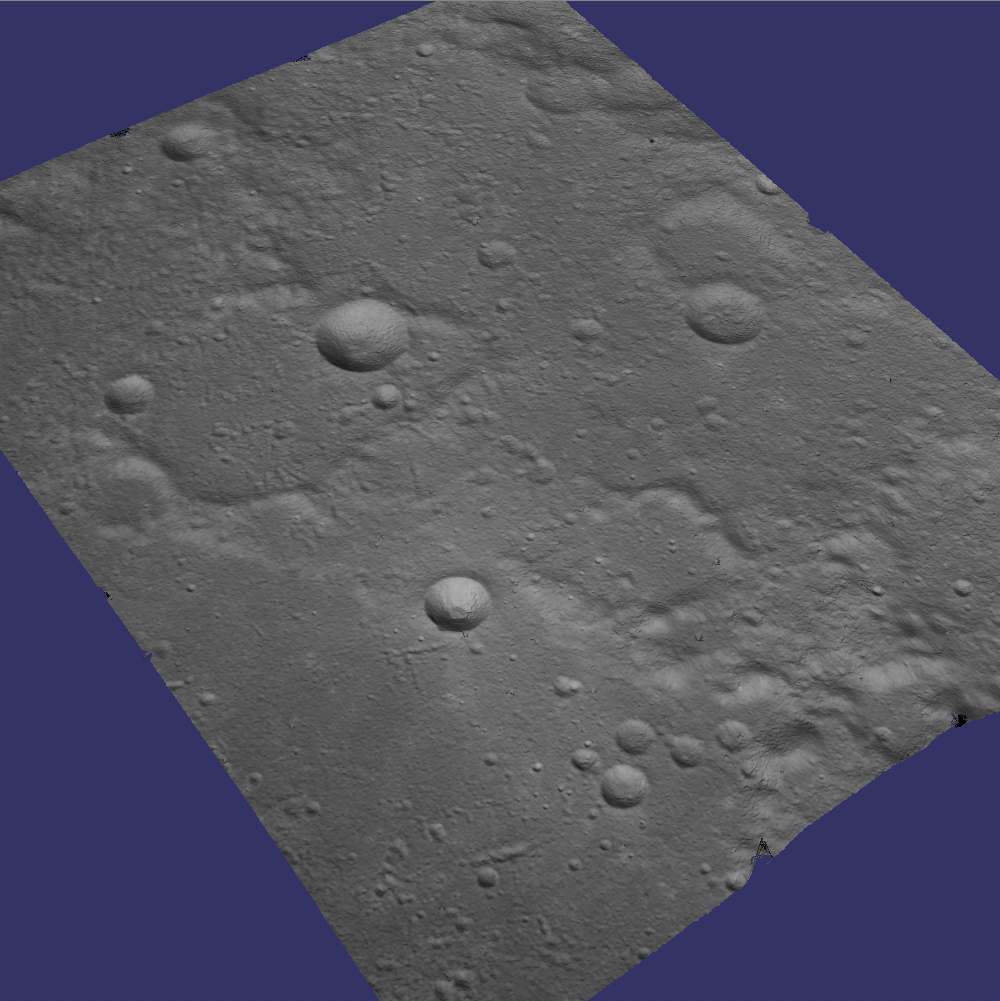
\includegraphics[width=3in]{images/examples/metric/metric_example.png}}
  \hfil
  \subfigure[{\tt KML Screenshot}]{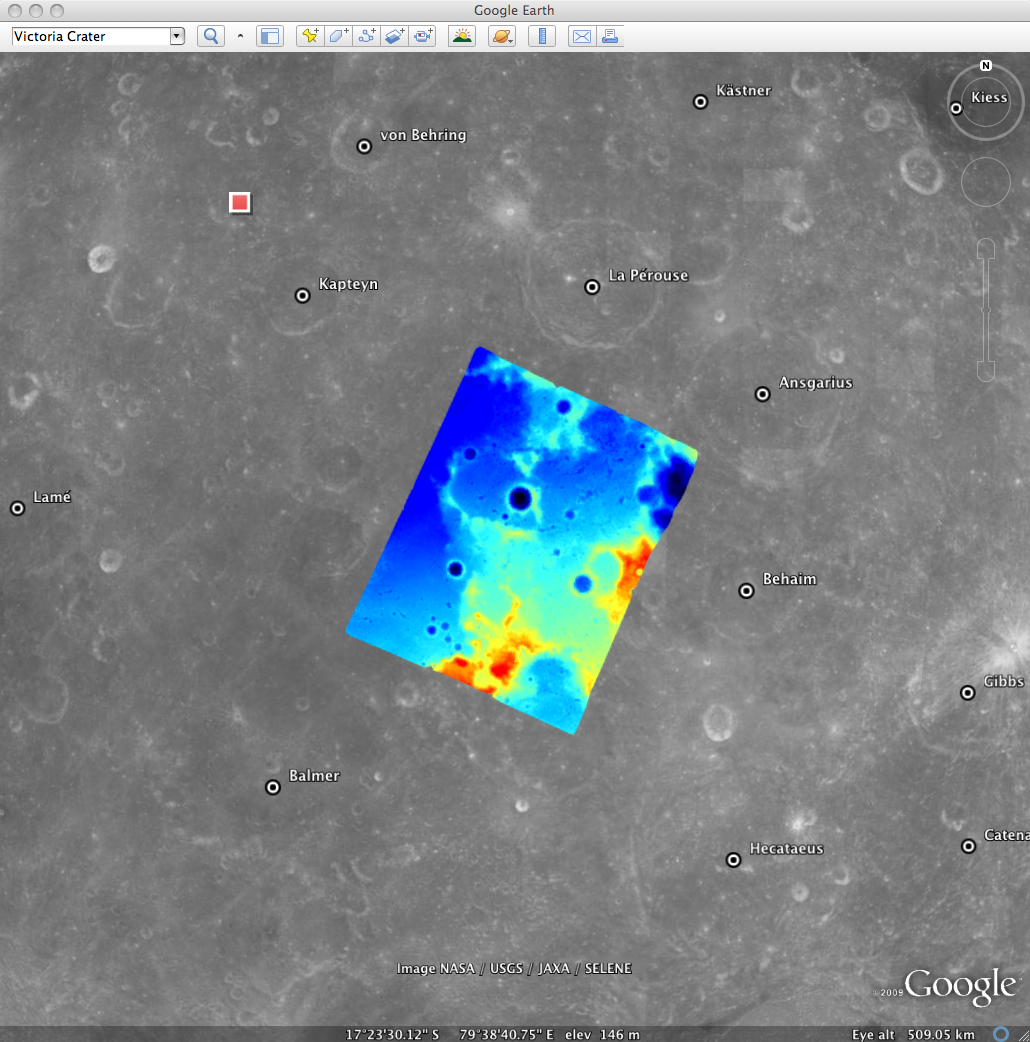
\includegraphics[width=3in]{images/examples/metric/metric_ge_example.png}}
\caption{Example output possible with Apollo Metric frames.}
\label{fig:metric_example}
\end{figure}

\subsubsection*{Commands}

\begin{verbatim}
    % Process tif files with not yet released commands %
    reduce from=AS15-M-2380.cub to=sub4-AS15-M-2380.cub sscale=4 lscale=4
    reduce from=AS15-M-2381.cub to=sub4-AS15-M-2381.cub sscale=4 lscale=4
    spiceinit from=sub4-AS15-M-2380.cub
    spiceinit from=sub4-AS15-M-2381.cub
    ipfind --max 10000 sub4*.cub
    ipmatch -i 50 -r homography sub4*.cub
    mkdir result
    stereo sub4-AS15-M-2380.cub sub4-AS15-M-2381.cub result/output
\end{verbatim}

\subsubsection*{Stereo Default}

\begin{verbatim}
    ### PREPROCESSING

    DO_INTERESTPOINT_ALIGNMENT 1
    INTERESTPOINT_ALIGNMENT_SUBSAMPLING 0
    DO_EPIPOLAR_ALIGNMENT 0

    FORCE_USE_ENTIRE_RANGE 1
    DO_INDIVIDUAL_NORMALIZATION 0

    PREPROCESSING_FILTER_MODE 3

    SLOG_KERNEL_WIDTH 1.5

    ### CORRELATION

    COST_MODE 2
    COST_BLUR 25

    H_KERNEL 35
    V_KERNEL 35

    H_CORR_MIN -250
    H_CORR_MAX 250
    V_CORR_MIN -70
    V_CORR_MAX 100

    SUBPIXEL_MODE 2

    SUBPIXEL_H_KERNEL 25
    SUBPIXEL_V_KERNEL 25

    # Hidden advanced function
    CORRSCORE_REJECTION_THRESHOLD 1.4

    ### FILTERING

    FILL_HOLES 1

    RM_H_HALF_KERN 5
    RM_V_HALF_KERN 5
    RM_MIN_MATCHES 60 # Units = percent
    RM_THRESHOLD 3
    RM_CLEANUP_PASSES 1

    ### DOTCLOUD

    NEAR_UNIVERSE_RADIUS 0.0
    FAR_UNIVERSE_RADIUS 0.0
\end{verbatim}

\section{Cassini ISS NAC}

\subsection{Enceladus}

\subsubsection*{Screenshot}

text

\subsubsection*{Commands}

text

\subsubsection*{Stereo Default}

text

\section{Lunar Reconaissance Orbiter LROC-NA}

\subsection{Lee-Lincoln Scarp}

This covers an area on the Moon called Taurus-Littrow valley where on
December 11, 1972 the astronauts of Apollo 17 landed. Though this
stereo pair doesn't contain the landing site, it is slightly west and
focusing on the Lee-Lincoln scarp that is on North Massif. The scarp
is an 80 m high feature that is the only visible sign of a deep fault.

\subsubsection*{Screenshot}

\begin{figure}[h!]
\centering
  \subfigure[{\tt 3D Rendering}]{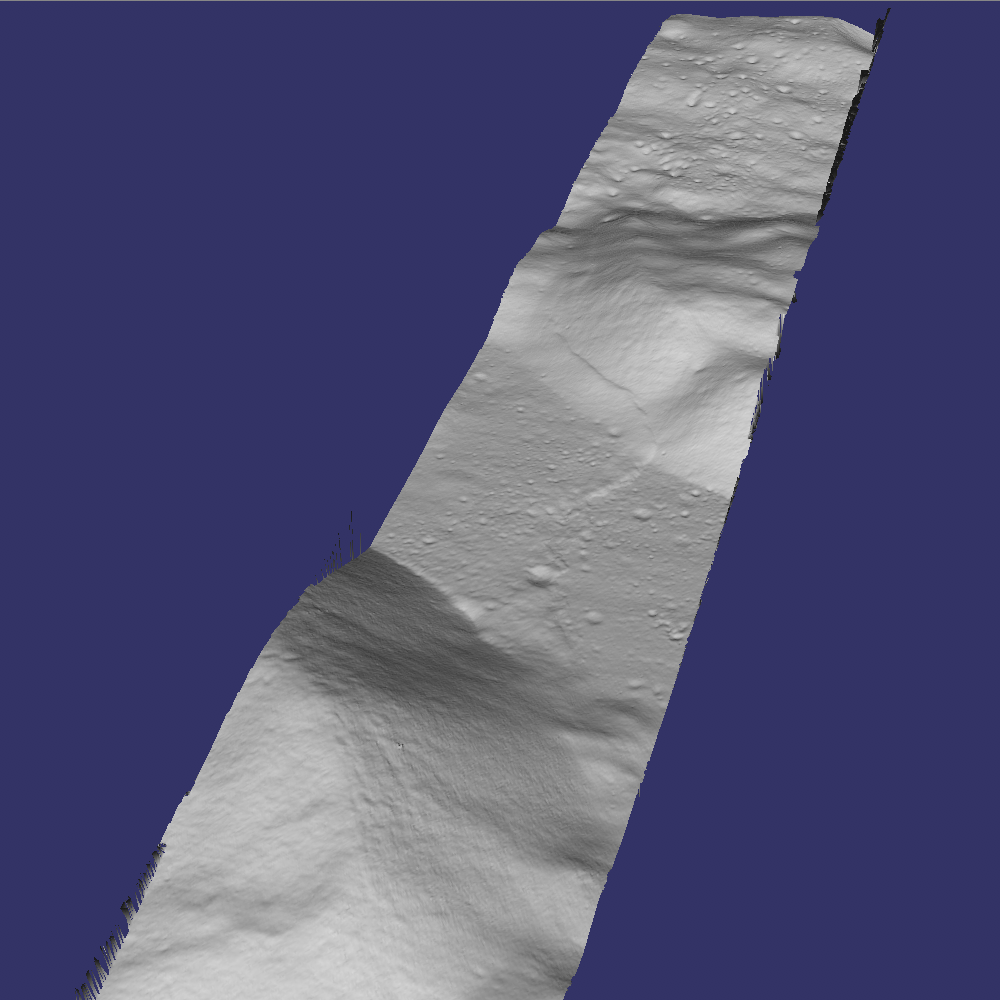
\includegraphics[width=3in]{images/examples/lrocna/lroc-na-example.png}}
  \hfil
  \subfigure[{\tt KML Screenshot}]{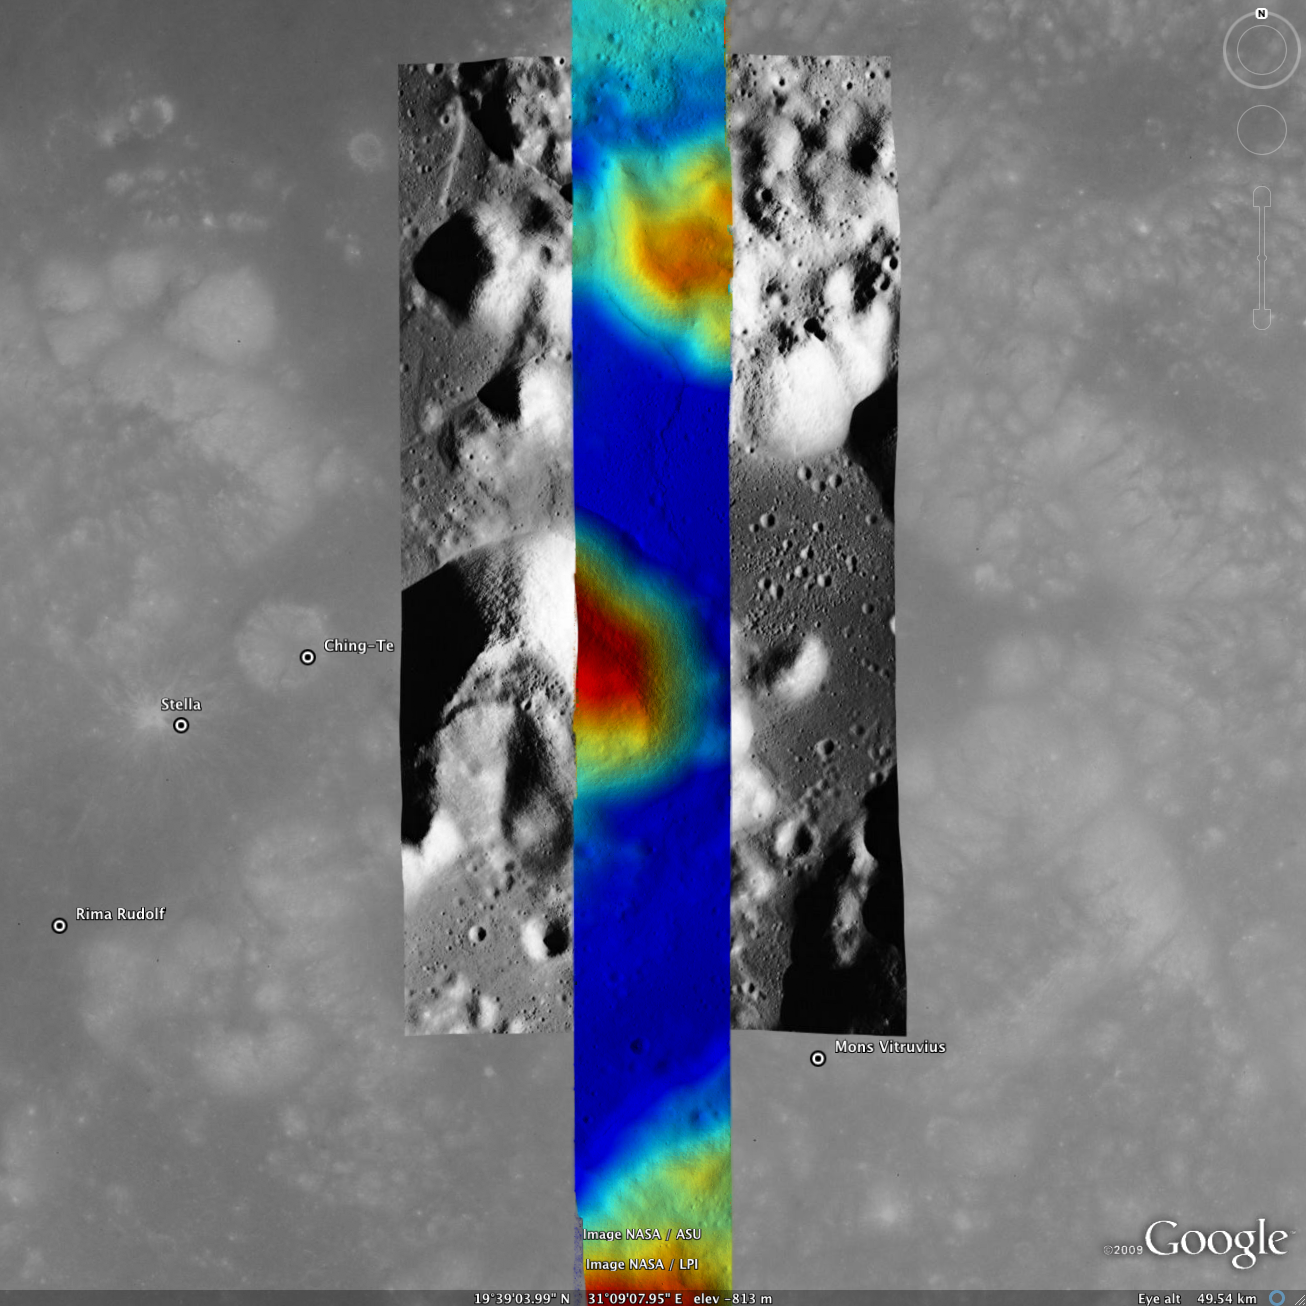
\includegraphics[width=3in]{images/examples/lrocna/lroc-na-ge_example.png}}
\caption{Example output possible with a LROC NA stereo pair, using only a single CCDs from observations.}
\label{fig:lroc-na-example}
\end{figure}

\subsubsection*{Commands}

\begin{verbatim}
    % Download nacl00002db8.* & nacl00004c86.*
    % process with unreleased tools to make cubes
    cam2map from=nacl00002db8.cub to=nacl00002db8.map.cub
    cam2map from=nacl00004c86.cub map=nacl00002db8.map.cub ...
            to=nacl00004c86.map.cub matchmap=true
    mkdir result
    stereo nacl00002db8.map.cub nacl00004c86.map.cub result/output
\end{verbatim}

\subsubsection*{Stereo Default}

\begin{verbatim}
    ### PREPROCESSING

    DO_INTERESTPOINT_ALIGNMENT 0
    INTERESTPOINT_ALIGNMENT_SUBSAMPLING 0
    DO_EPIPOLAR_ALIGNMENT 0

    FORCE_USE_ENTIRE_RANGE 1
    DO_INDIVIDUAL_NORMALIZATION 0

    PREPROCESSING_FILTER_MODE 2

    SLOG_KERNEL_WIDTH 1.5

    ### CORRELATION

    COST_BLUR 12
    COST_MODE 2

    H_KERNEL 29
    V_KERNEL 29

    H_CORR_MIN -425
    H_CORR_MAX 150
    V_CORR_MIN -100
    V_CORR_MAX 100

    SUBPIXEL_MODE 2

    SUBPIXEL_H_KERNEL 25
    SUBPIXEL_V_KERNEL 25

    ### FILTERING

    FILL_HOLES 1

    RM_H_HALF_KERN 5
    RM_V_HALF_KERN 5
    RM_MIN_MATCHES 60 # Units = percent
    RM_THRESHOLD 3
    RM_CLEANUP_PASSES 1

    ### DOTCLOUD

    NEAR_UNIVERSE_RADIUS 0.0
    FAR_UNIVERSE_RADIUS 0.0
\end{verbatim}

\section{Mars Global Surveyor MOC-NA}

In the Ames Stereo Pipeline tutorial we showed you how to process a
MOC-NA stereo pair that covered the Galaxius Fluctus channel. In this
section we plan to show you more examples but also to clear our
conscious. The tutorial picked a pristine pair that is not really
representative of typical MOC-NA stereo pairs. The Mars Global
Surveyor was particularly susceptible to a problem called spacecraft
'jitter'. All spacecraft to some degree wobble around a bit and this
causes wave-like distortions in linescan imagers. The cause of this
could be from the deployment of special antennae or the decay of
reaction wheels. Regardless, the MOC-NA pointing and position
information called SPICE does not show this jitter. This means that
the jitter will cause distortions in our pointcloud. The following
examples will show the typical distortions created by this problem.

It might concern you now that other missions will exhibit this
problem. Never fear, the science teams of HiRISE and LROC are aware of
your concern and are actively working on detecting and logging the
jitter in their respective SPICE data. The distortions will still
being in the raw imagery, but it won't cause artifacts in the
pointcloud or any following data product.

\subsection{Ceraunius Tholus}

Ceraunius Tholus is a steep volcano that is part of the Uranius group
on Mars. It can be found at 23.96N and 262.60 E. This DEM crosses the
volcano's caldera.

\subsubsection*{Screenshot}

\begin{figure}[h!]
\centering
  \subfigure[{\tt 3D Rendering}]{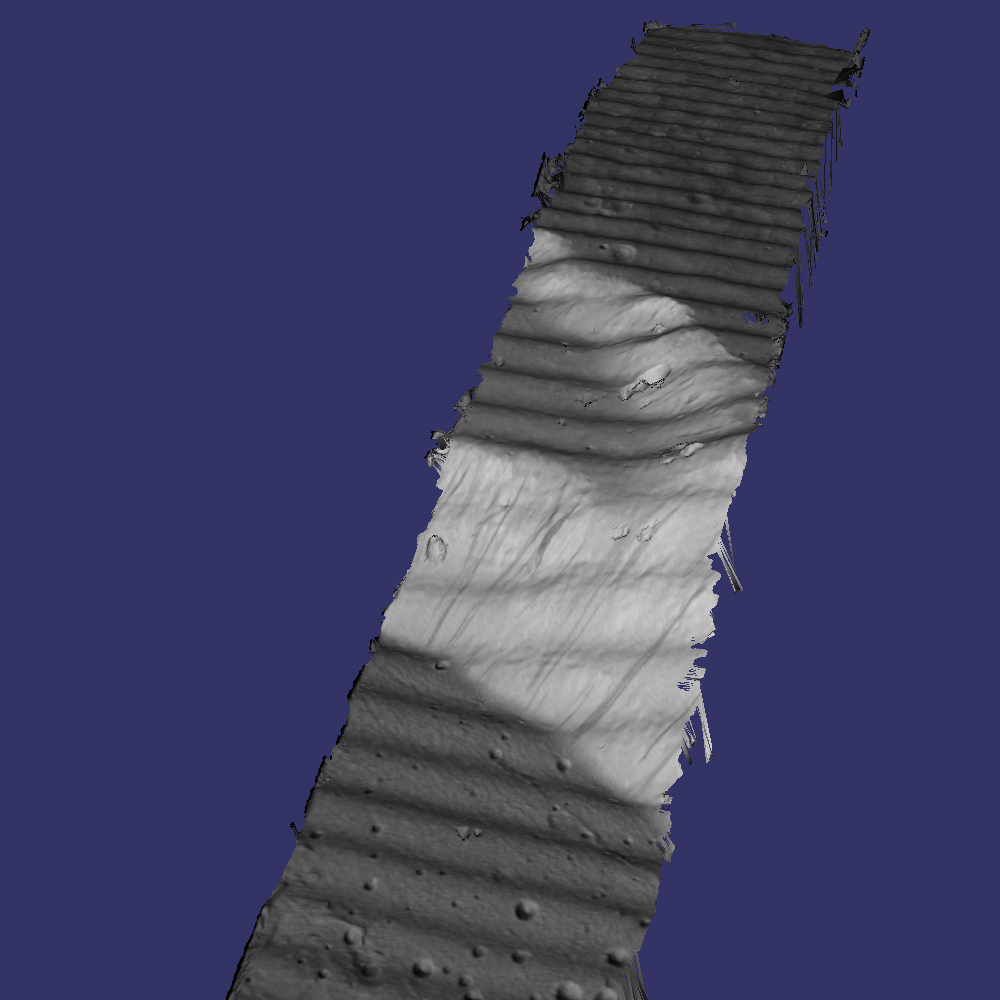
\includegraphics[width=3in]{images/examples/mocna/ceraunius_tholus_mocna.png}}
  \hfil
  \subfigure[{\tt KML Screenshot}]{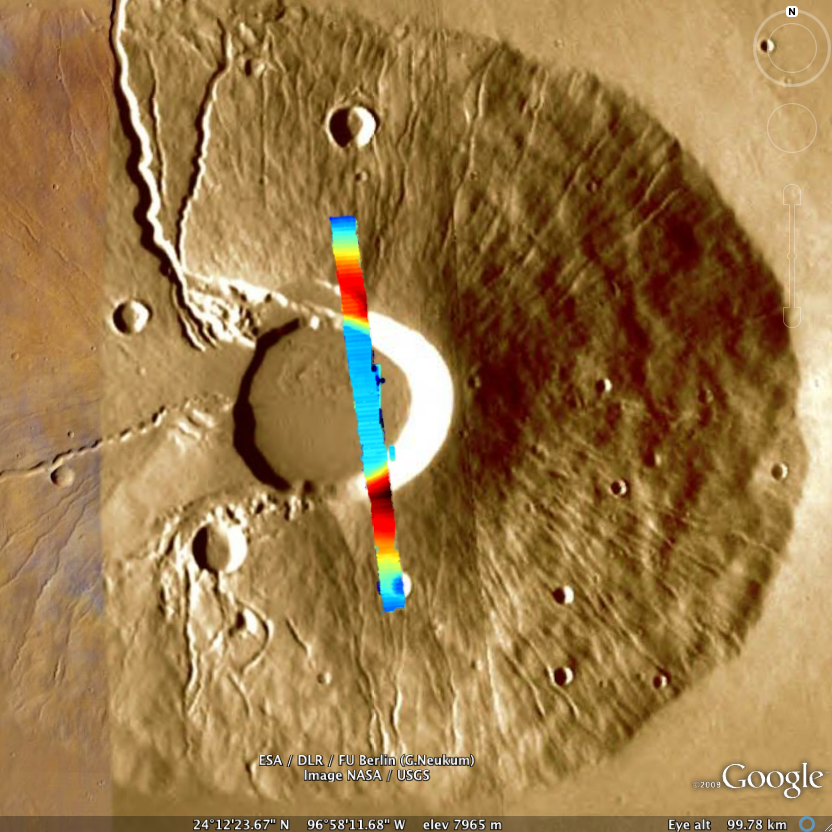
\includegraphics[width=3in]{images/examples/mocna/ceraunius_tholus_mocna_ge.png}}
\caption{Example output for MOC-NA of Ceraunius Tholus.}
\label{fig:mocna_ceraunius_example}
\end{figure}

\subsubsection*{Commands}

\begin{verbatim}
    % Download M0806047.img & R0701361.img
    moc2isis f=M0806047.img t=M0806047.cub mapping=no
    moc2isis f=R0701361.img t=R0701361.cub mapping=no
    cam2map from=M0806047.cub to=M0806047.map.cub
    cam2map from=R0701361.cub map=M0806047.map.cub to=R0701361.map.cub matchmap=true
    mkdir result
    stereo M0806047.map.cub R0701361.map.cub result/output
\end{verbatim}

\subsubsection*{Stereo Default}

\begin{verbatim}
    ### PREPROCESSING

    DO_INTERESTPOINT_ALIGNMENT 0
    INTERESTPOINT_ALIGNMENT_SUBSAMPLING 0
    DO_EPIPOLAR_ALIGNMENT 0

    FORCE_USE_ENTIRE_RANGE 1
    DO_INDIVIDUAL_NORMALIZATION 1

    PREPROCESSING_FILTER_MODE 2

    SLOG_KERNEL_WIDTH 1.5

    ### CORRELATION

    COST_BLUR 12
    COST_MODE 2

    H_KERNEL 25
    V_KERNEL 25

    H_CORR_MIN -12
    H_CORR_MAX 26
    V_CORR_MIN -50
    V_CORR_MAX 15

    SUBPIXEL_MODE 2

    SUBPIXEL_H_KERNEL 21
    SUBPIXEL_V_KERNEL 21

    ### FILTERING

    FILL_HOLES 1

    RM_H_HALF_KERN 5
    RM_V_HALF_KERN 5
    RM_MIN_MATCHES 60 # Units = percent
    RM_THRESHOLD 3
    RM_CLEANUP_PASSES 1

    ### DOTCLOUD

    NEAR_UNIVERSE_RADIUS 0.0
    FAR_UNIVERSE_RADIUS 0.0
\end{verbatim}

\subsection{North Tharsis}

The Malin Space Science System's website describes this image as the
`Throughs and terraces in northern Tharsis'. This DEM is located at
20.20 N and 118.18 W on Mars.

\subsubsection*{Screenshot}

\begin{figure}[h!]
\centering
  \subfigure[{\tt 3D Rendering}]{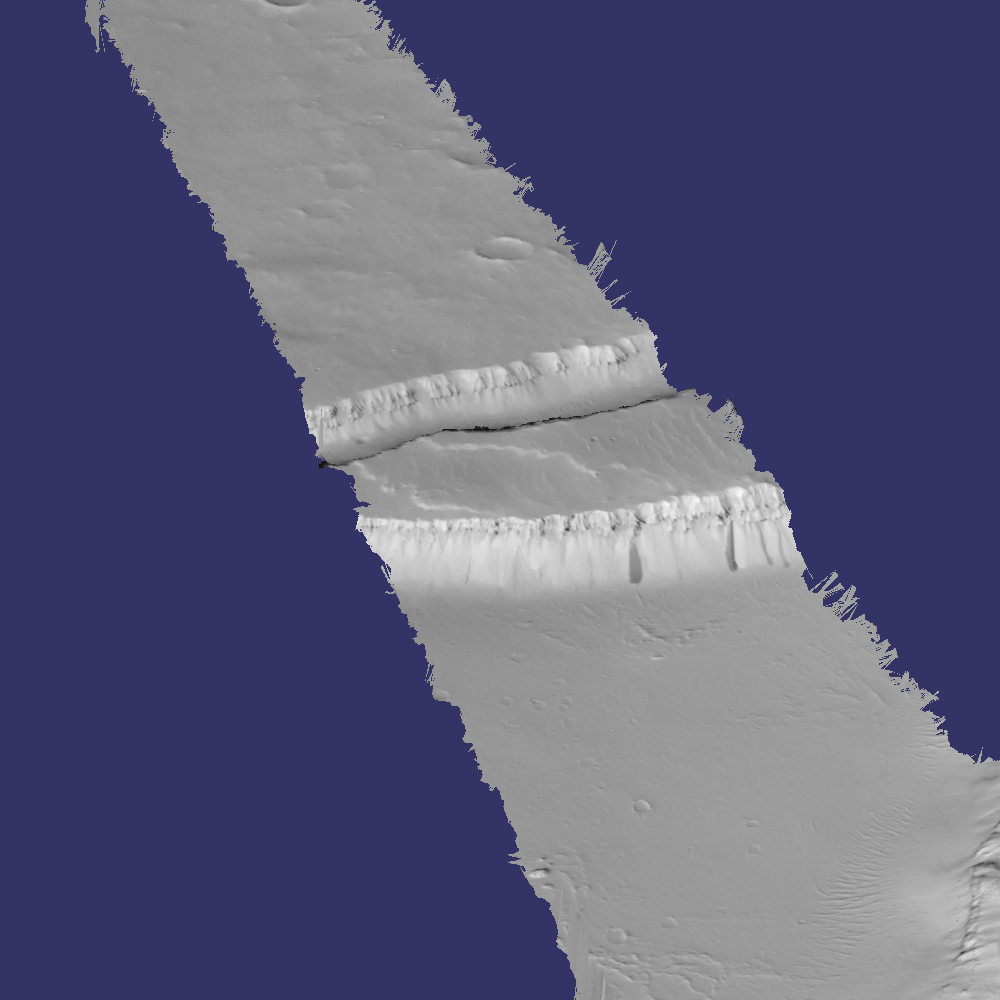
\includegraphics[width=3in]{images/examples/mocna/n_tharsis_mocna.png}}
  \hfil
  \subfigure[{\tt KML Screenshot}]{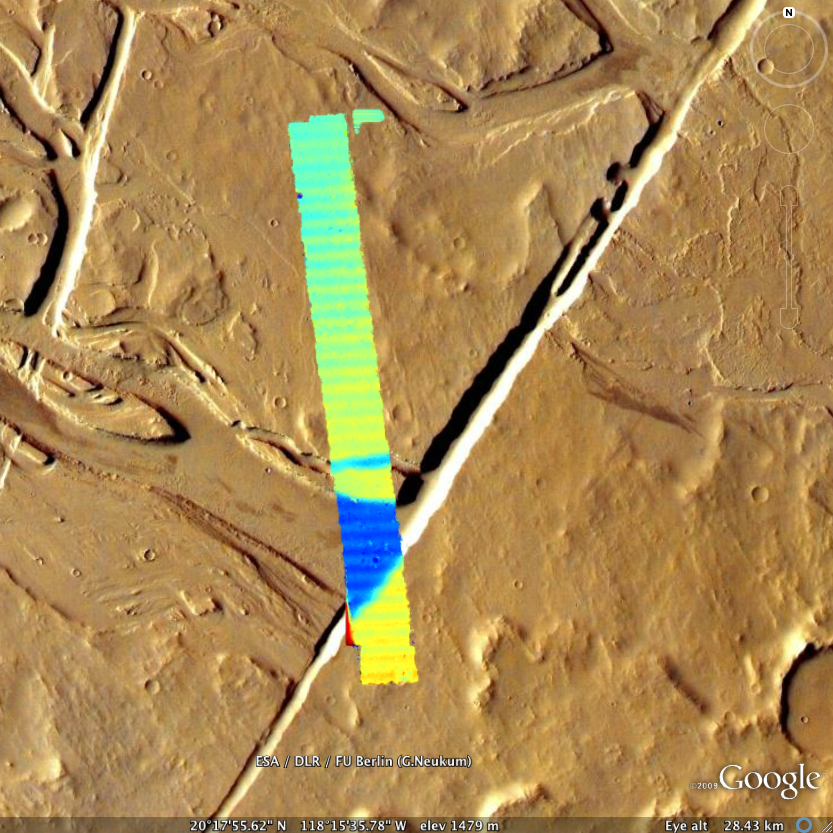
\includegraphics[width=3in]{images/examples/mocna/n_tharsis_mocna_ge.png}}
\caption{Example output for MOC-NA of North Tharsis.}
\label{fig:mocna_n_tharsis_example}
\end{figure}

\subsubsection*{Commands}

\begin{verbatim}
    % Download M0803097.img & S0701420.img
    moc2isis f=M0803097.img t=M0803097.cub mapping=no
    moc2isis f=S0701420.img t=S0701420.cub mapping=no
    cam2map from=M0803097.cub to=M0803097.map.cub
    cam2map from=S0701420.cub map=M0803097.map.cub to=S0701420.map.cub matchmap=true
    mkdr result
    stereo M0803097.map.cub S0701420.map.cub result/output
\end{verbatim}

\subsubsection*{Stereo Default}

\begin{verbatim}
    ### PREPROCESSING

    DO_INTERESTPOINT_ALIGNMENT 0
    INTERESTPOINT_ALIGNMENT_SUBSAMPLING 0
    DO_EPIPOLAR_ALIGNMENT 0

    FORCE_USE_ENTIRE_RANGE 1
    DO_INDIVIDUAL_NORMALIZATION 1

    PREPROCESSING_FILTER_MODE 2

    SLOG_KERNEL_WIDTH 1.5

    ### CORRELATION

    COST_BLUR 12
    COST_MODE 2

    H_KERNEL 25
    V_KERNEL 25

    H_CORR_MIN -50
    H_CORR_MAX 0
    V_CORR_MIN -85
    V_CORR_MAX 0

    SUBPIXEL_MODE 2

    SUBPIXEL_H_KERNEL 21
    SUBPIXEL_V_KERNEL 21

    ### FILTERING

    FILL_HOLES 1

    RM_H_HALF_KERN 5
    RM_V_HALF_KERN 5
    RM_MIN_MATCHES 60 # Units = percent
    RM_THRESHOLD 3
    RM_CLEANUP_PASSES 1

    ### DOTCLOUD

    NEAR_UNIVERSE_RADIUS 0.0
    FAR_UNIVERSE_RADIUS 0.0
\end{verbatim}

\section{Mars Reconaissance Orbiter CTX}

\subsection{North Terra Meridiani}

\subsubsection*{Screenshot}

\begin{figure}[h!]
\centering
  \subfigure[{\tt 3D Rendering}]{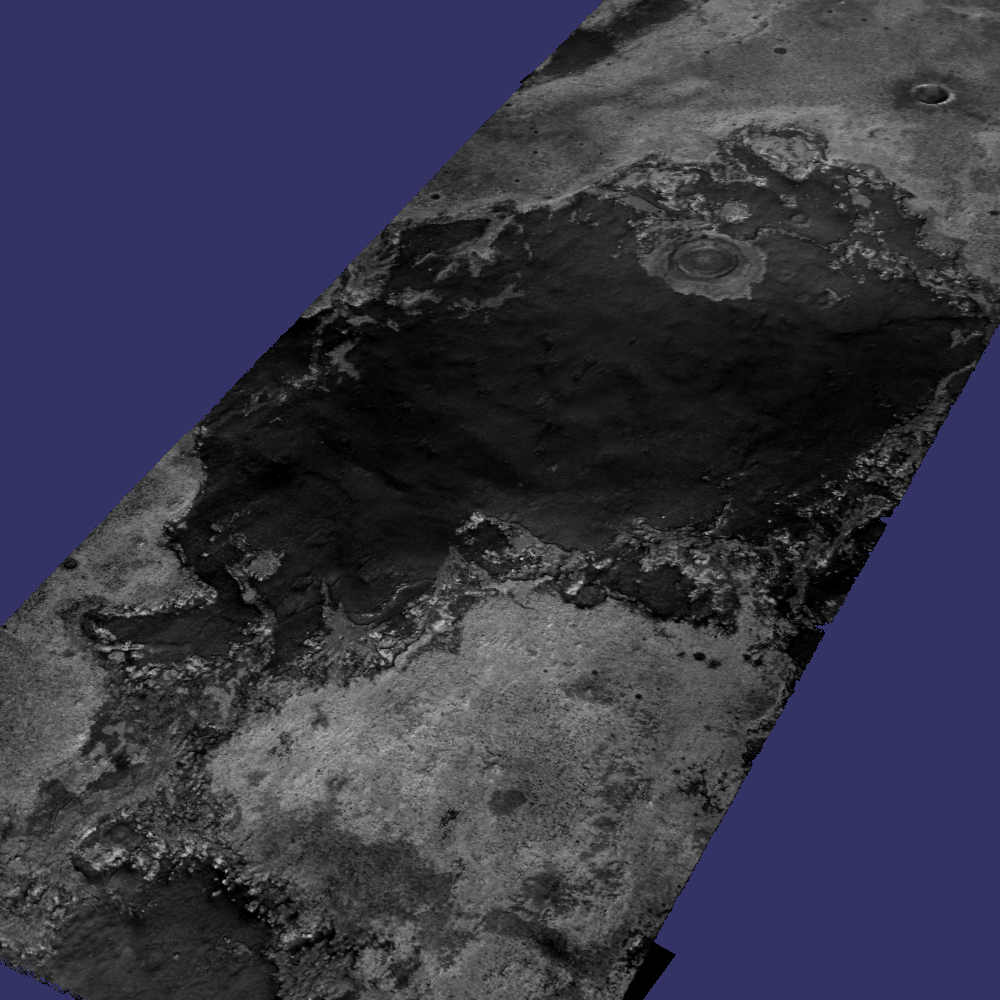
\includegraphics[width=3in]{images/examples/ctx/n_terra_meridiani_ctx.png}}
  \hfil
  \subfigure[{\tt KML Screenshot}]{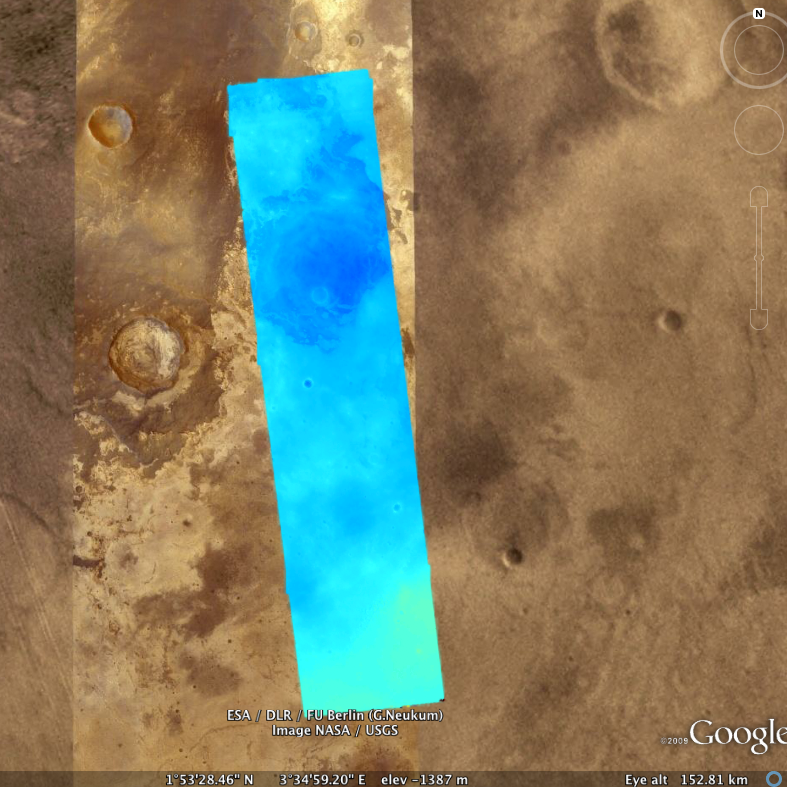
\includegraphics[width=3in]{images/examples/ctx/n_terra_meridiani_ctx_ge.png}}
\caption{Example output possible with the CTX imager aboard MRO.}
\label{fig:ctx_example}
\end{figure}

\subsubsection*{Commands}

\begin{verbatim}
    % Download P02_001981_1823_XI_02N356W.IMG &
    %          P03_002258_1817_XI_01N356W.IMG
    mroctx2isis from=P02_001981_1823_XI_02N356W.IMG to=P02_001981_1823_XI_02N356W.cub
    mroctx2isis from=P03_002258_1817_XI_01N356W.IMG to=P03_002258_1817_XI_01N356W.cub
    spiceinit from=P02_001981_1823_XI_02N356W.cub
    spiceinit from=P03_002258_1817_XI_01N356W.cub
    ctxcal from=P02_001981_1823_XI_02N356W.cub to=P02_001981_1823_XI_02N356W.cal.cub
    ctxcal from=P03_002258_1817_XI_01N356W.cub to=P03_002258_1817_XI_01N356W.cal.cub
    cam2map from=P02_001981_1823_XI_02N356W.cal.cub to=P02_001981_1823_XI_02N356W.map.cub
    cam2map from=P03_002258_1817_XI_01N356W.cal.cub to=P03_002258_1817_XI_01N356W.map.cub
\end{verbatim}

\subsubsection*{Stereo Default}

\begin{verbatim}
    ### PREPROCESSING

    DO_INTERESTPOINT_ALIGNMENT 1
    INTERESTPOINT_ALIGNMENT_SUBSAMPLING 0
    DO_EPIPOLAR_ALIGNMENT 0

    FORCE_USE_ENTIRE_RANGE 0
    DO_INDIVIDUAL_NORMALIZATION 0

    PREPROCESSING_FILTER_MODE 3

    SLOG_KERNEL_WIDTH 1.5

    ### CORRELATION

    COST_BLUR 0
    COST_MODE 2

    H_KERNEL 35
    V_KERNEL 35

    H_CORR_MIN -300
    H_CORR_MAX 300
    V_CORR_MIN -150
    V_CORR_MAX 150

    SUBPIXEL_MODE 3

    SUBPIXEL_H_KERNEL 21
    SUBPIXEL_V_KERNEL 21

    ### FILTERING

    FILL_HOLES 1

    RM_H_HALF_KERN 5
    RM_V_HALF_KERN 5
    RM_MIN_MATCHES 60 # Units = percest
    RM_THRESHOLD 3
    RM_CLEANUP_PASSES 1

    ### DOTCLOUD

    NEAR_UNIVERSE_RADIUS 0.0
    FAR_UNIVERSE_RADIUS 0.0
\end{verbatim}

\section{Mars Reconaissance Orbiter HiRISE}

HiRISE is one of the most challenging cameras to make 3D models
from. This is because HiRISE exposures can be several GiBs each and
working with this data requires patience as it will take time.

One important fact to know about HiRISE is that it is composed of
multiple linear CCDs that are arranged side by side with some vertical
offset. Their vertical offsets from each other on the image plane
means that the CCDs will view some of the same terrain but at a
slightly different time and a slightly different angle. Mosiacing the
CCDs together to a single image is not a simple process and involves
living with some imperfections.

We recommend at this time mosiacing CCDs via a script provided by
USGS. Having said that, we are also providing an alternative script
that will take raw HiRISE images and produce a mosaic a while
later. Both scripts take all red CCDs and project them via {\tt
  noproj} into the perspective of RED5. From there, {\tt hijitreg} is
performed to work out the relative offsets between CCDs. Finally the
CCDs are mosiaced together using the average offset listed from {\tt
  hijitreg} using the {\tt handmos} command. Below is an outline of
what our script does and is modelled after the tutorial provided by
USGS's Isis website.

\begin{verbatim}
    command outline
\end{verbatim}

Finally we recommend map projecting the product and normalizing the
stereo pair together. Notice that we map project the second image to
the map settings and crop of the first image. This means the images
will share the same origin and {\tt stereo's} search range should be
centered around zero.

\begin{verbatim}
    cam2map f=first.cub t=first.map.cub
    cam2map f=second.cub map=first.map.cub t=second.map.cub matchmap=true
    bandnorm f=first.map.cub t=first.norm.cub
    bandnorm f=second.map.cub t=second.norm.cub
    ls first.norm.cub second.norm.cub > fromlist
    ls first.norm.cub > holdlist
    equalizer fromlist=fromlist holdlist=holdlist
    mkdir result
    stereo first.norm.equ.cub second.norm.equ.cub result/output
\end{verbatim}

In the future, it is our understanding that the HiRISE team would like
to produce non-map-projected imagery from the PDS. When that happens,
most of the above commands will no longer be required.

\subsection{Columbia Hills}

The description is taken and modified from the HiRISE instrument website.
\url{http://hirise.lpl.arizona.edu/PSP_001513_1655}

\begin{quotation}
This HiRISE image shows the landing site of the Mars Exploration Rover
Spirit. The impact crater in the upper left-hand portion of the image
is "Bonneville Crater," which was investigated by Spirit shortly after
landing. In the lower right-hand portion of the image is "Husband
Hill," a large hill that Spirit climbed and where it spent much of its
now nearly three-year mission.

The bright irregularly-shaped feature in the area north-west of
Bonneville Crater is Spirit's parachute, now lying on the Martian
surface. Near the parachute is the cone-shaped "backshell" that helped
protect Spirit's lander during its seven-month journey to Mars. The
backshell appears relatively undamaged by its impact with the martian
surface. Wrinkles and folds in the parachute fabric are clearly
visible.

Immediately south west of Bonneville Crater shows Spirit's lander. The
crater in the upper left-hand portion of the image, just to the
northwest of the lander, is the one that the Mars Exploration Rover
team named "Sleepy Hollow."

The north rim of Bonneville Crater shows the damaged remnant of the
heat shield that protected the vehicle during the high-speed entry
through the Martian atmosphere. The heat shield impacted the surface
after being separated from the vehicle during the final stages of the
descent.

South of Husband Hill shows the current location of Spirit. Toward the
top of the image is "Home Plate," a plateau of layered rocks that
Spirit explored during the early part of its third year on
Mars. Spirit itself is clearly seen just to the southeast of Home
Plate. Also visible are the tracks made by the rover before it arrived
at its current location.

Written by: Steve Squyres
\end{quotation}

\subsubsection*{Screenshot}

\begin{figure}[h!]
\centering
  \subfigure[{\tt 3D Rendering}]{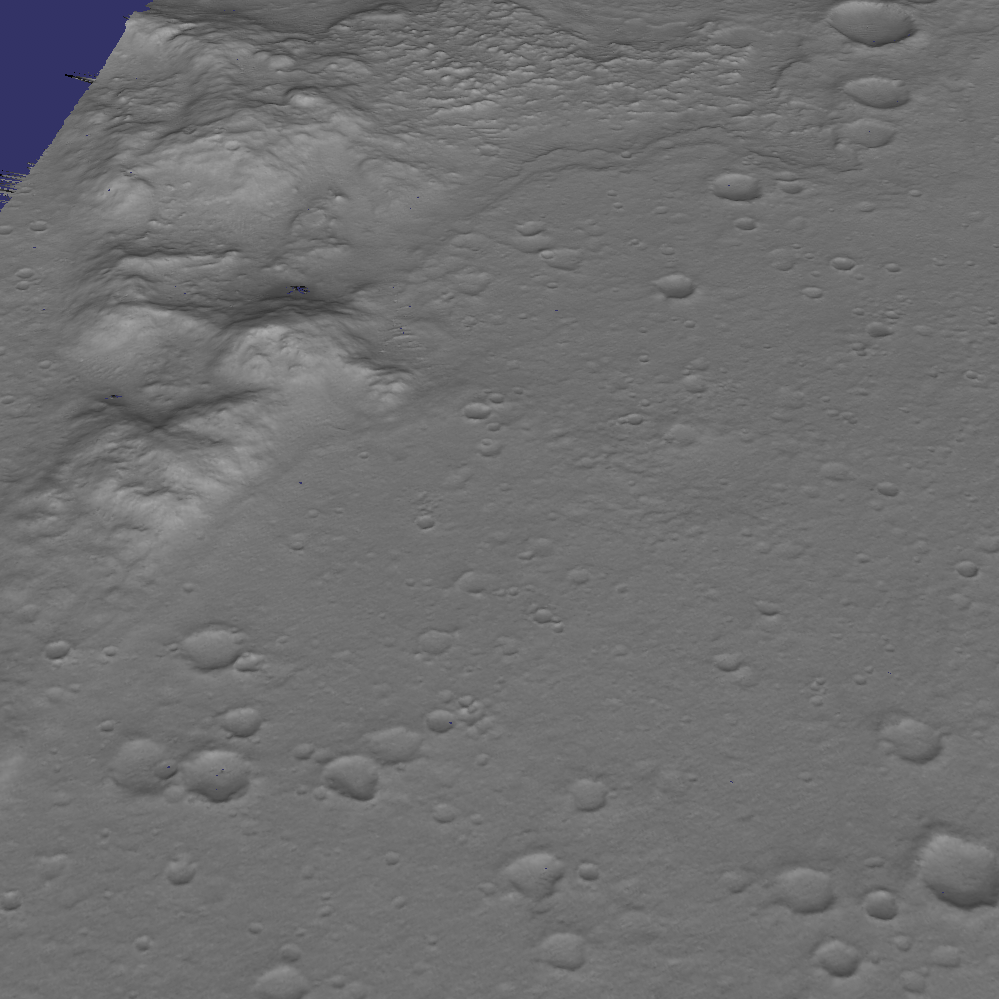
\includegraphics[width=3in]{images/examples/hirise/chills_hirise_example.png}}
  \hfil
  \subfigure[{\tt KML Screenshot}]{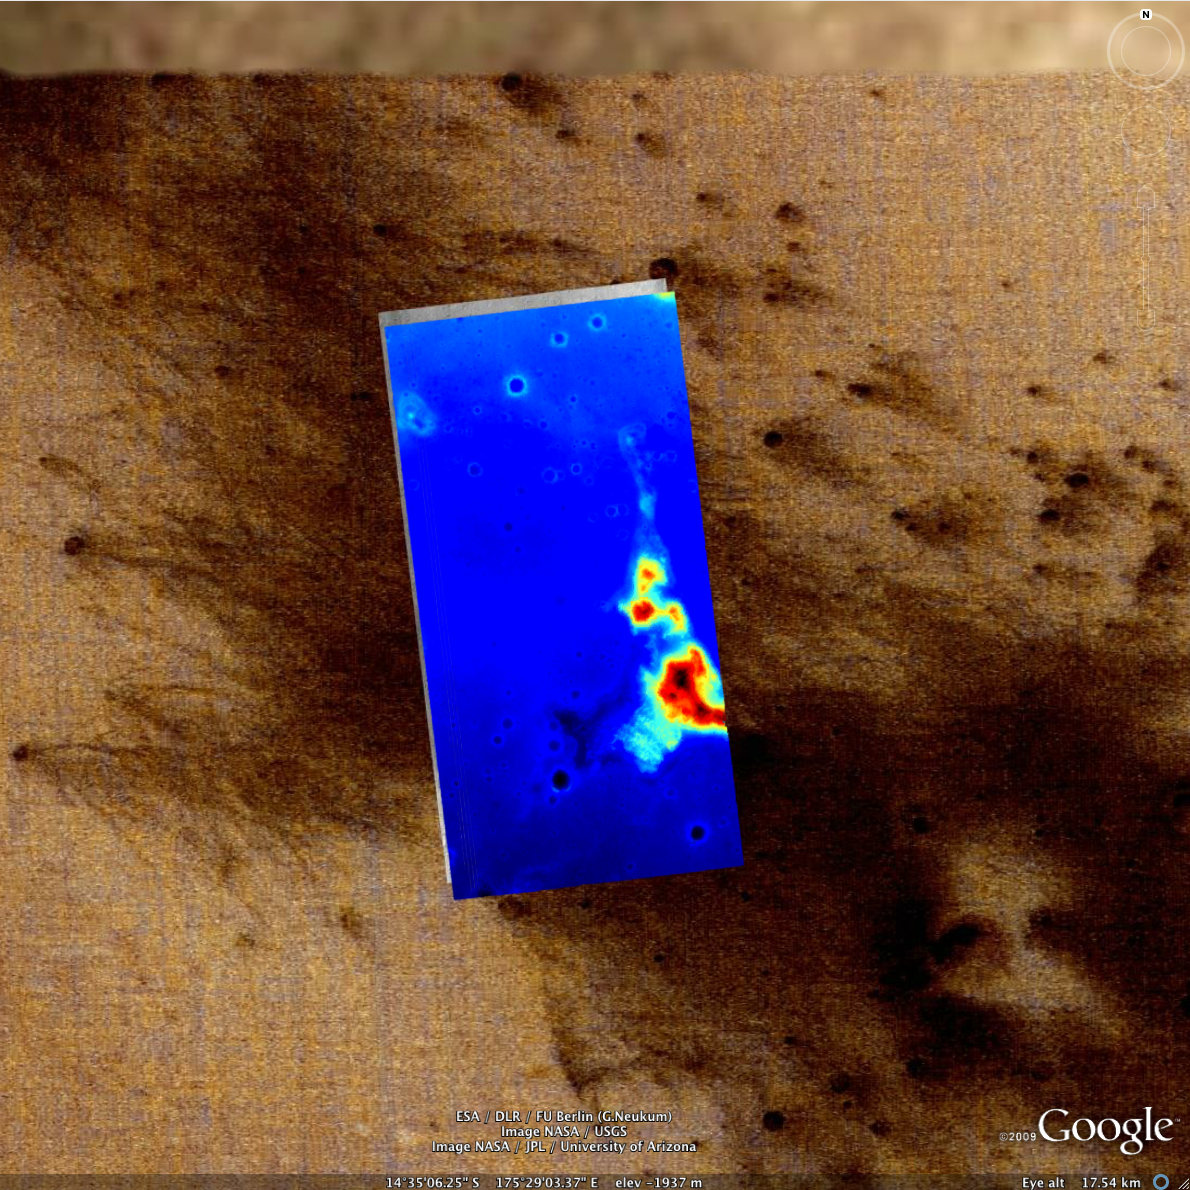
\includegraphics[width=3in]{images/examples/hirise/chills_hirise_ge_example.png}}
\caption{Example output using HiRISE data of East Mareotis Tholus.}
\label{fig:hirise_chills_example}
\end{figure}

\subsubsection*{Commands}

\begin{verbatim}
    % Download all of the RED IMG for PSP_001513_1655 & %
    %                                 PSP_001777_1650   %
    ~/HiRISE_stitch.py PSP_001513_1655_RED0_0.IMG
    ~/HiRISE_stitch.py PSP_001777_1650_RED0_0.IMG
    cam2map from=PSP_001513_1655_REDmosaic.norm.cub to=PSP_001513_1655_REDmosaic.map.cub
    cam2map from=PSP_001777_1650_REDmosaic.norm.cub map=PSP_001513_1655_REDmosaic.map.cub ...
            to=PSP_001777_1650_REDmosaic.norm.cub matchmap=true
    bandnorm from=PSP_001513_1655_REDmosaic.map.cub to=PSP_001513_1655_REDmosaic.map.norm.cub
    bandnorm from=PSP_001777_1650_REDmosaic.map.cub to=PSP_001777_1650_REDmosaic.map.norm.cub
    ls *.map.norm.cub > fromlist
    ls *1513*.map.norm.cyb > holdlist
    equalizer fromlist=fromlist holdlist=holdlist
    rm *REDmosaic.map.norm.cub *REDmosaic.map.cub
    mkdir result
    stereo PSP_001513_1655.map.norm.equ.cub PSP_001777_1650.map.norm.equ.cub result/output
\end{verbatim}

\subsubsection*{Stereo Default}

\begin{verbatim}
    ### PREPROCESSING

    DO_INTERESTPOINT_ALIGNMENT 0
    INTERESTPOINT_ALIGNMENT_SUBSAMPLING 0
    DO_EPIPOLAR_ALIGNMENT 0

    FORCE_USE_ENTIRE_RANGE 1
    DO_INDIVIDUAL_NORMALIZATION 0

    PREPROCESSING_FILTER_MODE 2

    SLOG_KERNEL_WIDTH 1.5

    ### CORRELATION

    COST_MODE 0
    COST_BLUR 0

    H_KERNEL 50
    V_KERNEL 50

    H_CORR_MIN 210
    H_CORR_MAX 450
    V_CORR_MIN -320
    V_CORR_MAX 320

    SUBPIXEL_MODE 2

    SUBPIXEL_H_KERNEL 25
    SUBPIXEL_V_KERNEL 25

    ### FILTERING

    FILL_HOLES 1

    RM_H_HALF_KERN 5
    RM_V_HALF_KERN 5
    RM_MIN_MATCHES 60 # Units = percent
    RM_THRESHOLD 3
    RM_CLEANUP_PASSES 1

    ### DOTCLOUD

    NEAR_UNIVERSE_RADIUS 0.0
    FAR_UNIVERSE_RADIUS 0.0
\end{verbatim}

\subsection{East Mareotis Tholus}

The description is taken from the HiRISE instrument website.
\url{http://hirise.lpl.arizona.edu/PSP_001760_2160}

\begin{quotation}
East Mareotis Tholus is a small volcano in Tempe Terra, Mars. This
area is on the northeast edge of the Tharsis bulge that was built up
by many large and small volcanoes.

One of the many questions we hope to address with HiRISE is the
relative roles of the giant shield volcanoes (such as Olympus Mons)
and smaller volcanic features (such as East Mareotis Tholus).

The anaglyph covers 4.4 x 6.9 km (2.7 x 4.9 miles) and the topography
can be viewed using red-blue glasses. The elongated pit at the summit
of the volcano is where the lava issued forth. The large circular hole
just to the SW of the vent is an impact crater. The gouges in the
ground to the SE of the volcano are tectonic fissures (called graben)
that are now filled with sand dunes. The area is covered with large
amounts of wind-blown dust, so it is not surprising that lava flows
and other smaller volcanic features are not visible.

However, the smooth shape of the volcano, and the lack of lava layers
exposed in the impact crater, allow for the possiblity that this
volcano is composed largely of ash, rather than lava flows.

Written by: Laszlo P. Keszthelyi
\end{quotation}

\subsubsection*{Screenshot}

\begin{figure}[h!]
\centering
  \subfigure[{\tt 3D Rendering}]{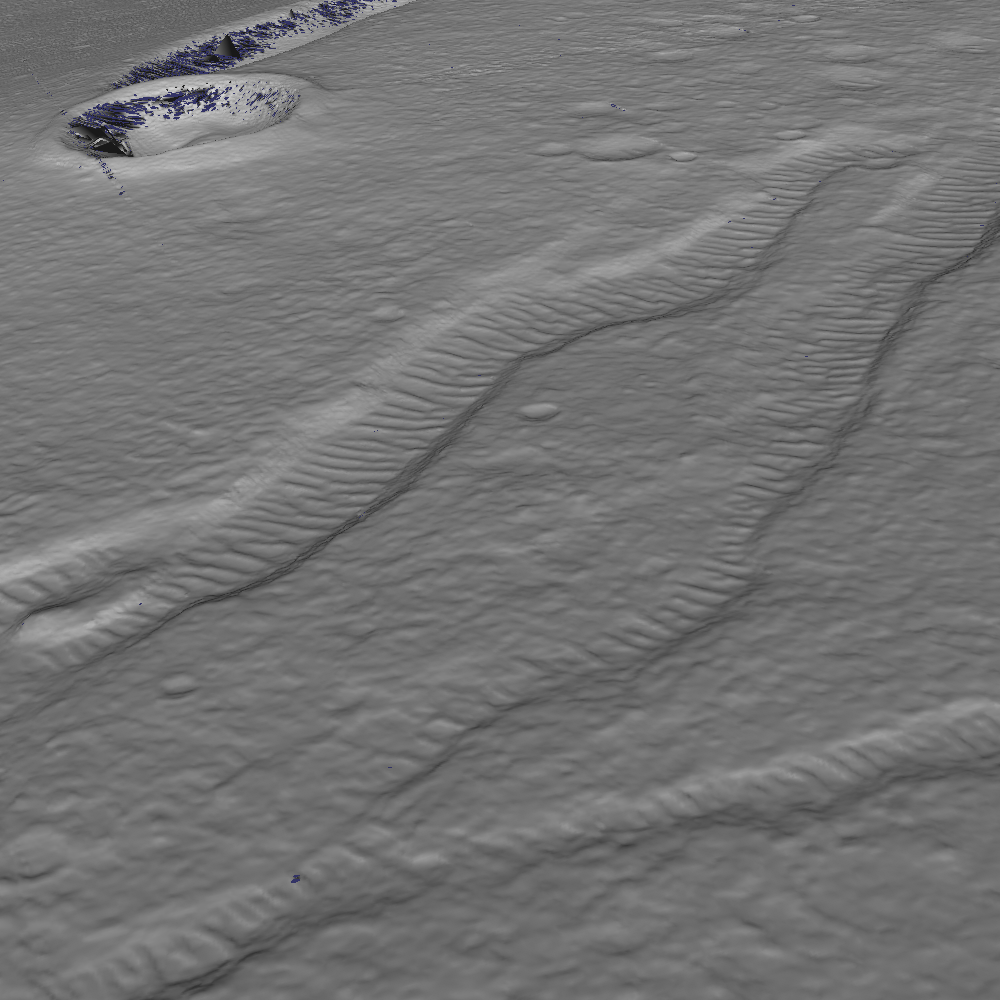
\includegraphics[width=3in]{images/examples/hirise/emare_example.png}}
  \hfil
  \subfigure[{\tt KML Screenshot}]{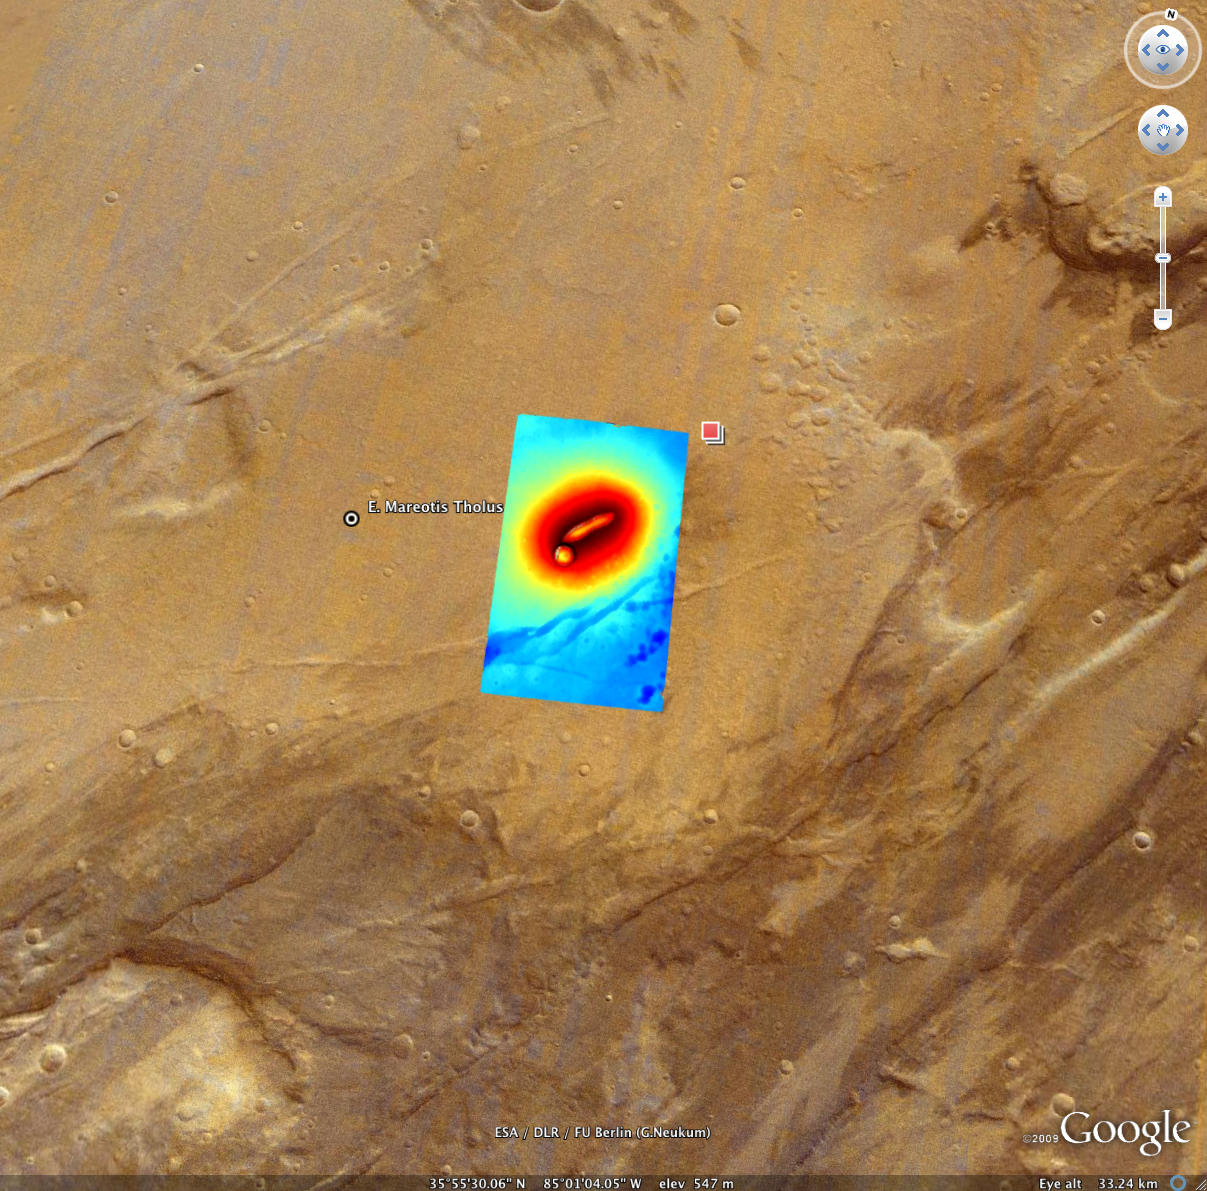
\includegraphics[width=3in]{images/examples/hirise/emare_ge_example.png}}
\caption{Example output using HiRISE data of East Mareotis Tholus.}
\label{fig:hirise_emare_example}
\end{figure}

\subsubsection*{Commands}

\begin{verbatim}
    % Download all of the RED IMG for PSP_001364_2160 & %
    %                                 PSP_001760_2160   %
    ~/HiRISE_stitch.py PSP_001364_2160_RED0_0.IMG
    ~/HiRISE_stitch.py PSP_001760_2160_RED0_0.IMG
    cam2map from=PSP_001364_2160_REDmosaic.norm.cub to=PSP_001364_2160_REDmosaic.map.cub
    cam2map from=PSP_001760_2160_REDmosaic.norm.cub map=PSP_001364_2160_REDmosaic.map.cub ...
            to=PSP_001760_2160_REDmosaic.map.cub matchmap=true
    bandnorm from=PSP_001364_2160_REDmosaic.map.cub to=PSP_001364_2160_REDmosaic.map.norm.cub
    bandnorm from=PSP_001760_2160_REDmosaic.map.cub to=PSP_001760_2160_REDmosaic.map.norm.cub
    ls *.map.norm.cub > fromlist
    ls *1760*.map.norm.cub > holdlist
    equalizer fromlist=fromlist holdlist=holdlist
    rm *REDmosaic.map.norm.cub *REDmosaic.map.cub
    mkdir result
    stereo PSP_001364_2160.map.norm.equ.cub PSP_001760_2160.map.norm.equ.cub result/output
\end{verbatim}

\subsubsection*{Stereo Default}

\begin{verbatim}
    ### PREPROCESSING

    DO_INTERESTPOINT_ALIGNMENT 0
    INTERESTPOINT_ALIGNMENT_SUBSAMPLING 0
    DO_EPIPOLAR_ALIGNMENT 0

    FORCE_USE_ENTIRE_RANGE 1
    DO_INDIVIDUAL_NORMALIZATION 0

    PREPROCESSING_FILTER_MODE 2

    SLOG_KERNEL_WIDTH 1.5

    ### CORRELATION

    COST_BLUR 0
    COST_MODE 0

    H_KERNEL 25
    V_KERNEL 25

    H_CORR_MIN -80
    H_CORR_MAX 150
    V_CORR_MIN -80
    V_CORR_MAX 50

    SUBPIXEL_MODE 0

    SUBPIXEL_H_KERNEL 25
    SUBPIXEL_V_KERNEL 25

    ### FILTERING

    FILL_HOLES 1

    RM_H_HALF_KERN 5
    RM_V_HALF_KERN 5
    RM_MIN_MATCHES 60 # Units = percest
    RM_THRESHOLD 3
    RM_CLEANUP_PASSES 1

    ### DOTCLOUD

    NEAR_UNIVERSE_RADIUS 0.0
    FAR_UNIVERSE_RADIUS 0.0
\end{verbatim}

\subsection{North Terra Meridiani Crop}

HiRISE website only has to say that this is `Layered Materials within
a Small Crater'. Hopefully you'll still agree that this is cool.

\subsubsection*{Screenshot}

\begin{figure}[h!]
\centering
  \subfigure[{\tt 3D Rendering}]{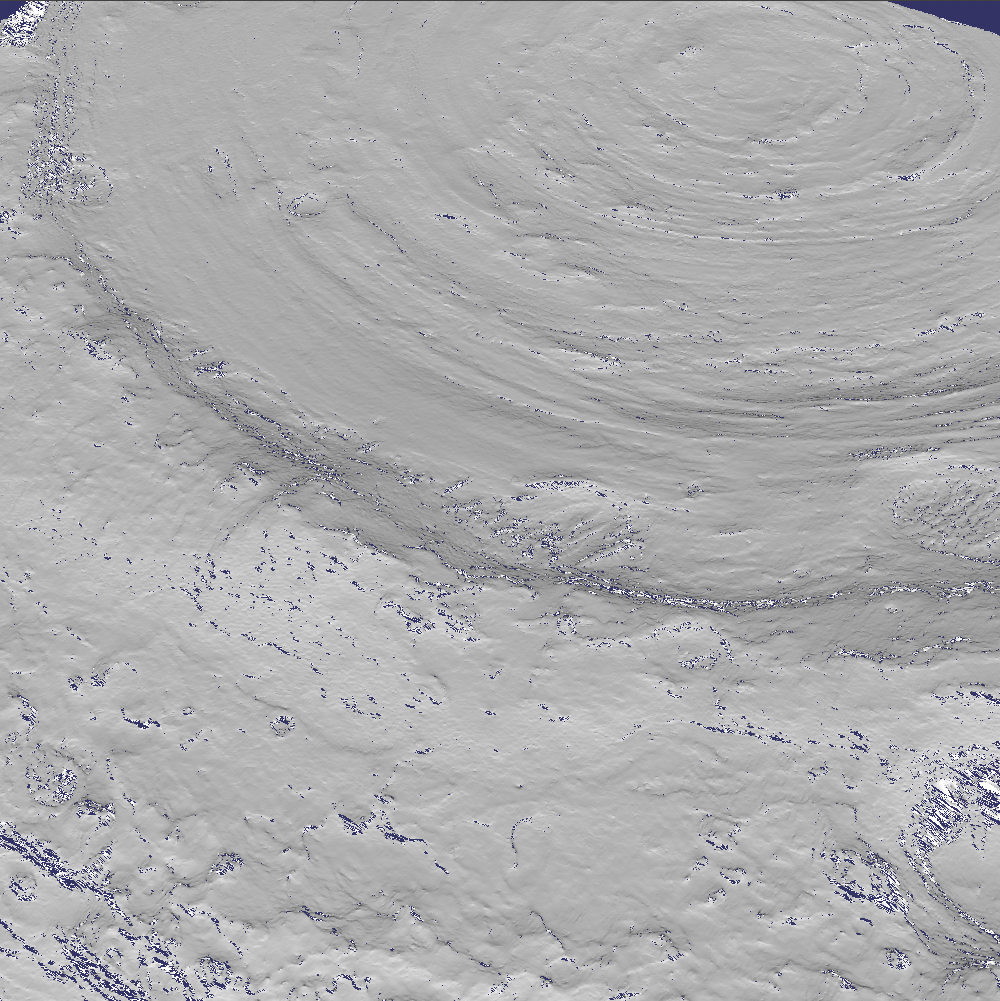
\includegraphics[width=3in]{images/examples/hirise/nterra_example.png}}
  \hfil
  \subfigure[{\tt KML Screenshot}]{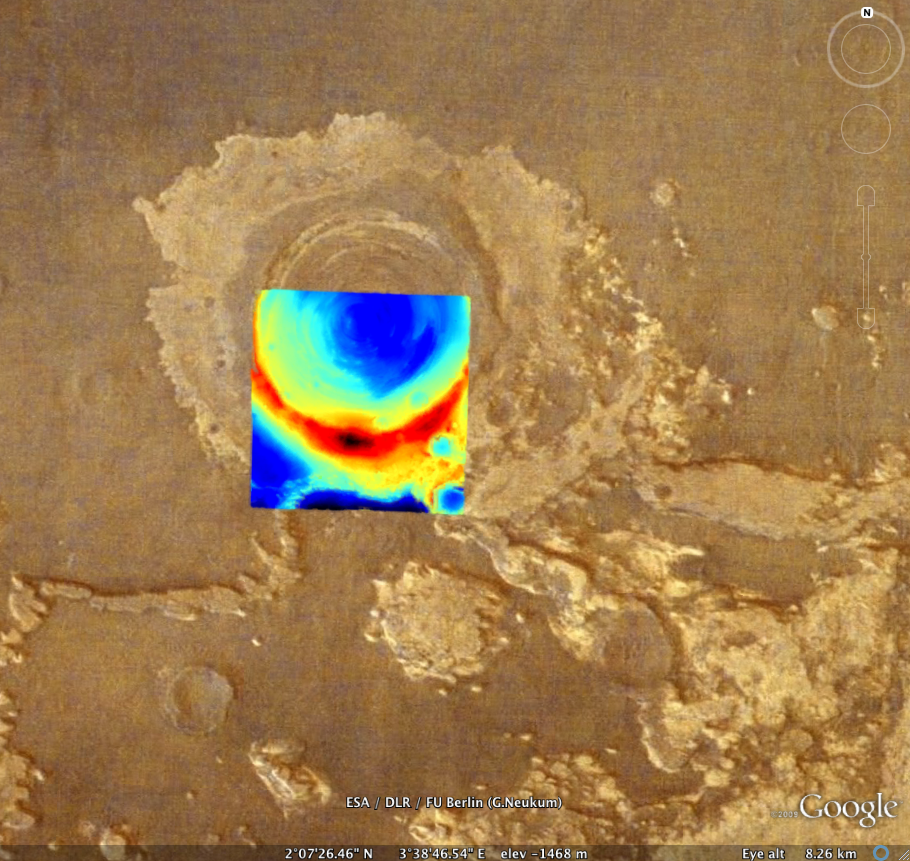
\includegraphics[width=3in]{images/examples/hirise/nterra_ge_example.png}}
\caption{Example output using cropped HiRISE data of North Terra Meridiani.}
\label{fig:hirise_nterra_example}
\end{figure}

\subsubsection*{Commands}

\begin{verbatim}
    % Download all of the IMG for PSP_001981_1825 & %
    %                             PSP_002258_1825   %
    ~/HiRISE_stitch.py PSP_001981_1825_RED0_0.IMG
    ~/HiRISE_stitch.py PSP_002258_1825_RED0_0.IMG
    cam2map from=PSP_001981_1825_REDmosaic.norm.cub to=PSP_001981_1825_REDmosaic.map.cub
    cam2map from=PSP_002258_1825_REDmosaic.norm.cub map=PSP_001981_1825_REDmosaic.map.cub ...
            to=PSP_002258_1825_REDmosaic.map.cub matchmap=true
    bandnorm from=PSP_001981_1825_REDmosaic.map.cub to=PSP_001981_1825_REDmosaic.map.norm.cub
    bandnorm from=PSP_002258_1825_REDmosaic.map.cub to=PSP_002258_1825_REDmosaic.map.norm.cub
    ls *.map.norm.cub > fromlist
    ls *1981*.map.norm.cub > holdlist
    equalizer fromlist=fromlist holdlist=holdlist
    crop from=PSP_001981_1825_REDmosaic.map.norm.equ.cub to=PSP_001981_1825.crop.cub ...
         sample=7497 line=41318 nsamp=10000 nline=10000
    crop from=PSP_002258_1825_REDmosaic.map.norm.equ.cub to=PSP_002258_1825.crop.cub ...
         sample=7982 line=41310 nsamp=10000 nline=10000
    rm *REDmosaic*.cub
    mkdir result
    stereo PSP_001981_1825.crop.cub PSP_002258_1825.crop.cub result/output
\end{verbatim}

\subsubsection*{Stereo Default}

\begin{verbatim}
    ### PREPROCESSING

    DO_INTERESTPOINT_ALIGNMENT 0
    INTERESTPOINT_ALIGNMENT_SUBSAMPLING 0
    DO_EPIPOLAR_ALIGNMENT 0

    FORCE_USE_ENTIRE_RANGE 1
    DO_INDIVIDUAL_NORMALIZATION 0

    PREPROCESSING_FILTER_MODE 2

    SLOG_KERNEL_WIDTH 1.5

    ### CORRELATION

    COST_BLUR 21
    COST_MODE 2

    H_KERNEL 45
    V_KERNEL 45

    H_CORR_MIN -270
    H_CORR_MAX -70
    V_CORR_MIN -14
    V_CORR_MAX 26

    SUBPIXEL_MODE 0

    SUBPIXEL_H_KERNEL 25
    SUBPIXEL_V_KERNEL 25

    ### FILTERING

    FILL_HOLES 1

    RM_H_HALF_KERN 5
    RM_V_HALF_KERN 5
    RM_MIN_MATCHES 60 # Units = percent
    RM_THRESHOLD 3
    RM_CLEANUP_PASSES 1

    ### DOTCLOUD

    NEAR_UNIVERSE_RADIUS 0.0
    FAR_UNIVERSE_RADIUS 0.0
\end{verbatim}

\section{MESSENGER MDIS}

This a proof of concept showing of the strength of building on top of
ISIS. MDIS data is not a goal for the designers but it does have a
camera model in ISIS. This alone means that it too can be processed by
the Ames Stereo Pipeline.

For future mappers it is suggested checking out Mercury Flyby 3 data
which was not available at the time of this writing. Flyby 3 and Flyby
2 seem to have covered some of the same terrain with the narrow angle
camera.

\subsection{Wide Angle on flyby 2}

Like most imagery coming from spacecraft that are currently not in
orbit with their target, it is very hard to find good stereo
pairs. This is taken from a single flyby from the same camera seconds
apart. It should also be noted that this pair is taken from different
wave lengths as well \emph{(The letter at the end of the file
  designates the current filter being used on the wide angle
  camera)}. Unfortunately theres not enough of a perspective change to
make anything other than the spherical surface.

\subsubsection*{Screenshot}

\begin{figure}[h!]
  \begin{center}
  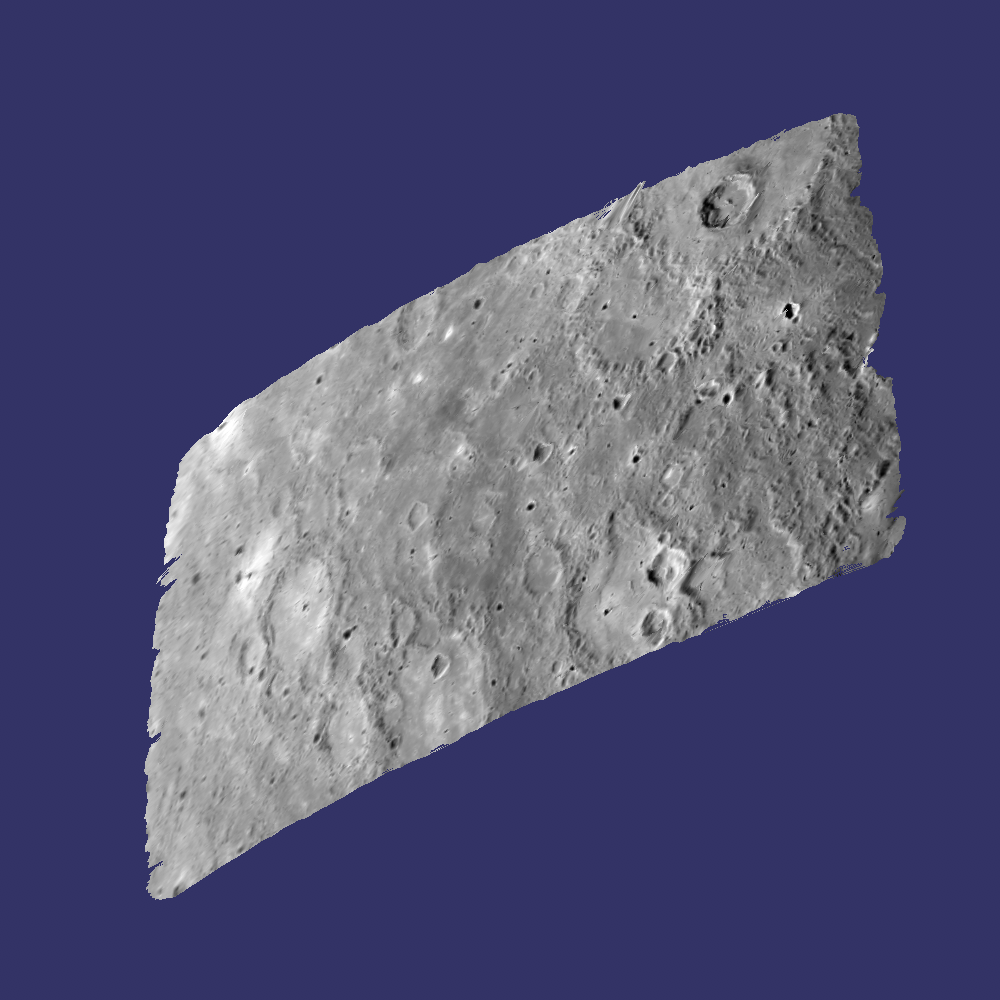
\includegraphics[width=5in]{images/examples/mdis/mdis_wide_example.png}
  \end{center}
  \caption{ A rough attempt at MDIS imagery }
  \label{fig:mdis_attempt}
\end{figure}

\subsubsection*{Commands}

\begin{verbatim}
    mdis2isis from=EW0108825359A.IMG to=EW0108825359A.cub
    mdis2isis from=EW0108825379C.IMG to=EW0108825379C.cub
    spiceinit from=EW0108825359A.cub
    spiceinit from=EW0108825359C.cub
    ipfind --max 10000 *.cub
    ipmatch -i 10 -r homography *.cub
    mkdir result
    stereo EW0108825359A.cub EW0108825379C.cub stereo/output
\end{verbatim}

\subsubsection*{Stereo Default}

\begin{verbatim}
    ### PREPROCESSING

    DO_INTERESTPOINT_ALIGNMENT 1
    INTERESTPOINT_ALIGNMENT_SUBSAMPLING 0
    DO_EPIPOLAR_ALIGNMENT 0

    FORCE_USE_ENTIRE_RANGE 0
    DO_INDIVIDUAL_NORMALIZATION 1

    PREPROCESSING_FILTER_MODE 2

    SLOG_KERNEL_WIDTH 1.5

    ### CORRELATION

    COST_BLUR 5
    COST_MODE 0

    H_KERNEL 25
    V_KERNEL 25

    H_CORR_MIN -10
    H_CORR_MAX 10
    V_CORR_MIN -2
    V_CORR_MAX 2

    SUBPIXEL_MODE 2

    SUBPIXEL_H_KERNEL 19
    SUBPIXEL_V_KERNEL 19

    ### FILTERING

    FILL_HOLES 1

    RM_H_HALF_KERN 5
    RM_V_HALF_KERN 5
    RM_MIN_MATCHES 60 # Units = percent
    RM_THRESHOLD 3
    RM_CLEANUP_PASSES 1

    ### DOTCLOUD

    NEAR_UNIVERSE_RADIUS 0.0
    FAR_UNIVERSE_RADIUS 0.0

\end{verbatim}
